\section{Mechanism Experiments}
\label{app:mechanism}
\subsection{Projection-Blind Synthetic Validation of the Bias--Variance Trade-off}
\label{sec:synthetic}

We isolate the statistical effect of compression in a controlled Gaussian sequence estimation problem that is \emph{projection-blind}: the target is generated independently of the projection matrix, so that no favorable alignment or artificial mismatch is built into the ground truth.
The target's energy \emph{profile}, in contrast, is deliberately controlled---heavy-tailed here and dense Gaussian in Appendix~\ref{sec:synthetic_failure}---to instantiate the recoverable and diffuse off-subspace regimes that the theory distinguishes.
The mixture is used only to generate a problem instance.
Specifically, independently for each coordinate, we draw
$b_j\sim\operatorname{Bernoulli}(\pi)$,
$g_j\sim\mathcal N(0,1)$, and $T_j\sim t_\nu$, and set
\begin{equation}
\Theta_j^\star
=
(1-b_j)\tau_0g_j
+
b_j\tau_1\sqrt{\frac{\nu-2}{\nu}}\,T_j .
\label{eq:synthetic_gt}
\end{equation}
The factor $\sqrt{(\nu-2)/\nu}$ standardizes $T_j$ to unit variance, so $\tau_1$ is the standard deviation---not the scale parameter---of the heavy-tailed component.
We use $\pi=0.01$, $\tau_0=0.005$, $\tau_1=0.5$, and $\nu=3$.
This zero-mean i.i.d.\ problem-generation law is isotropic with
\begin{equation}
v
=
\mathbb E_{\mathcal Q}[(\Theta_j^\star)^2]
=
(1-\pi)\tau_0^2+\pi\tau_1^2
=
2.52475\times10^{-3}.
\label{eq:synthetic_target_energy}
\end{equation}
Using seed 13, we draw one realization $\theta^\star$ of $\Theta^\star$ and an independent $P$ and hold both fixed across all noise levels and all $M=200$ trials.
Only the observation noise is resampled:
$y^{(m)}=\theta^\star+(\sigma_y/\sqrt{n_{\mathrm{eff}}})\epsilon^{(m)}$ with
$\epsilon^{(m)}\sim\mathcal N(0,I_D)$.
Thus, in every trial, the same realized vector $\theta^\star$ remains the population optimum; the mixture describes variation across possible synthetic problem instances, whereas Proposition~\ref{prop:energy_noise} additionally averages over that generation law.
Each method solves the constrained least-squares problem
\(\hat{\theta}_{\mathcal S}=\arg\min_{\theta\in\mathcal S}\frac{1}{2}\|y-\theta\|_2^2\),
with \(\mathcal S=\mathbb{R}^D\) for LoRA, \(\mathcal S=\mathrm{col}(P)\) for Uni-LoRA, and the sparse-augmented space \(\mathrm{col}([P,E_{\mathcal I}])\) for ProLoSA, whose support \(\mathcal I\) is the top-\(K\) coordinates of the post-warmup residual \(|y-PP^\top y|\)---the estimation-setting analog of the warmup SNIP score in Eq.~\eqref{eq:warmup_snip_score}---and we measure the population excess risk \(\frac{1}{2}\|\hat{\theta}-\theta^\star\|_2^2\).
We use \(D=4096\), \(d=16\), \(K=32\), and \(n_{\mathrm{eff}}=512\) (full configuration in Appendix~\ref{app:exp_details}); the realized mixture draw has \(33\) heavy-tailed coordinates, and the largest \(32\) residual coordinates carry \(98.8\%\) of the off-subspace energy.

Figure~\ref{fig:synthetic_validation} reveals the predicted transition between variance- and bias-dominated regimes. 
The risk of full-space LoRA grows rapidly with \(\sigma_y\) because its unconstrained estimator retains noise in all \(D\) coordinates, whereas Uni-LoRA suppresses estimation variance but pays a projection-bias floor since the independently generated \(\theta^\star\) need not lie in \(\mathrm{col}(P)\). 
Uni-LoRA is therefore worse than LoRA at small noise but preferable once the full-space variance grows large---exactly the crossover of Eq.~\eqref{eq:compression_condition}.
For the fixed realized target and projection,
$\hat v_\perp=\|(I-PP^\top)\theta^\star\|_2^2/(D-d)=2.6486\times10^{-3}$.
Equation~\eqref{eq:conditional_compressed_risk} therefore predicts the exact conditional crossover
$\sigma_y^\ast=\sqrt{n_{\mathrm{eff}}\hat v_\perp}=1.165$, matching the observed intersection in Figure~\ref{fig:synthetic_validation}A.
The overall realized energy $\|\theta^\star\|_2^2/D=2.6444\times10^{-3}$ is nearly identical because $P$ is independent and $D$ is large, but it is $\hat v_\perp$, rather than the ensemble quantity $v$, that gives the fixed-instance threshold.

Panels B--C make the mechanism explicit via the empirical decomposition
\(\mathrm{Bias}=\frac{1}{2}\|\bar{\theta}-\theta^\star\|_2^2\)
and
\(\mathrm{Variance}=\frac{1}{2M}\sum_{m}\|\hat{\theta}^{(m)}-\bar{\theta}\|_2^2\)
across the \(M\) noise realizations, where \(\bar{\theta}\) is the mean estimate.
Both components use the same fixed $(\theta^\star,P)$ and the same $M$ estimates. With denominator $M$ in the empirical variance, their sum equals the empirical mean excess risk exactly; the plug-in bias includes finite-$M$ estimation noise.

\paragraph{Conditioning and aggregation.}
A repeated training/noise trial does not draw a new optimum. If a separate experiment changes the target to $\theta_t^\star$, we first compute its own conditional mean $\mu_t=\mathbb E[\hat\theta\mid t]$, bias $B_t=\tfrac12\|\mu_t-\theta_t^\star\|^2$, and variance $V_t=\tfrac12\mathbb E[\|\hat\theta-\mu_t\|^2\mid t]$. A declared task average may report $\mathbb E_t[B_t+V_t]$, but estimates from distinct targets must not be pooled into a single fixed-target decomposition. In particular, pooled estimator dispersion includes variation of $\mu_t$ across tasks; adding it to an independently averaged conditional bias double-counts or misattributes variability. Concentrated and diffuse targets, different target strengths, and different source distributions are therefore separate experiments. Random supports, when used, contribute to estimator variability conditional on the fixed target. The matched-budget and dense-failure curves below follow this convention throughout the noise sweep.

\paragraph{Conditional sequence results.}
At \(\sigma_y=0.5\), LoRA has essentially no bias but incurs an excess risk of \(1.00\) almost entirely from variance; Uni-LoRA reduces this variance to nearly zero but its projection bias raises the total risk to \(5.41\); ProLoSA corrects the mismatch and reaches \(0.08\). 
At \(\sigma_y=1.5\), the variance of LoRA drives its risk to \(9.00\), Uni-LoRA remains at its bias floor of \(5.44\), and ProLoSA attains a risk of only \(0.47\).
Sparse correction thus recovers most of the approximation error without giving up the variance-reduction benefit of compression---precisely because the off-subspace energy of the heavy-tailed target is concentrated on a few large coordinates, the recoverable case identified in Appendix~\ref{sec:when_fails}.

\paragraph{Matched-budget comparison.}
The comparison above spends $d+K=48$ parameters for ProLoSA against $d=16$ for Uni-LoRA, so it demonstrates bias reduction but not yet the matched-budget claim of Proposition~\ref{prop:matched_budget}.
Figure~\ref{fig:synthetic_matched_budget} therefore fixes the total budget at $B=d+K=48$ and compares, on the identical fixed target and noise realizations, a compressed-only estimator of dimension $B$ against hybrids ($d=16$, $K=32$) whose supports are random, noise-dependent (top-$K$ residual, the SNIP analog), or oracle (top-$K$ of the true off-subspace residual).
Here ``oracle'' means that the support may inspect the fixed target $\theta^\star$; the top-$K$ rule is a target-informed surrogate, not an exhaustive search over all size-$K$ supports.
The results are consistent with both parts of the proposition.
First, the random hybrid nearly ties the $B$-dimensional compressed-only estimator across the entire noise range (e.g., $5.37$ vs.\ $5.36$ at $\sigma_y=0.5$ and $5.46$ vs.\ $5.45$ at $\sigma_y=1.5$); the fixed $B$-dimensional projection has a conditional bias floor of $5.349$, close to both curves.
This is the high-dimensional single-instance counterpart of Corollary~\ref{cor:random_support}, whose equality is an ensemble expectation under the isotropic target law.
Second, informed supports win by orders of magnitude on this concentrated target ($0.08$ at $\sigma_y=0.5$), because the target-informed top-$K$ directions recover more energy than the realized bias difference between the $d$- and $B$-dimensional projections (Eq.~\eqref{eq:fixed_matched_budget_condition}): their coordinates contain $98.8\%$ of the residual's coordinatewise energy, and projection onto the resulting augmented subspace removes $99.0\%$ of the projection bias.
The same panel also quantifies the selection-variance effect of the remark after Proposition~\ref{prop:matched_budget}: the noise-dependent support tracks the oracle at small $\sigma_y$ but degrades relative to it as noise grows ($0.47$ vs.\ $0.16$ at $\sigma_y=1.5$), while still improving over compressed-only by an order of magnitude.
Finally, comparing the full-space estimator with the $B=48$ compressed-only estimator answers the budget-level question of when compression itself pays.
Denoting that fixed $B$-dimensional projection by $P_B$,
$\hat v_{\perp,B}=\|(I-P_BP_B^\top)\theta^\star\|_2^2/(D-B)=2.6427\times10^{-3}$, so Eq.~\eqref{eq:conditional_compressed_risk} predicts
$\sigma_y^\ast=\sqrt{n_{\mathrm{eff}}\hat v_{\perp,B}}=1.163$, matching the observed crossing near $1.16$.

\begin{figure*}[t]
    \centering
    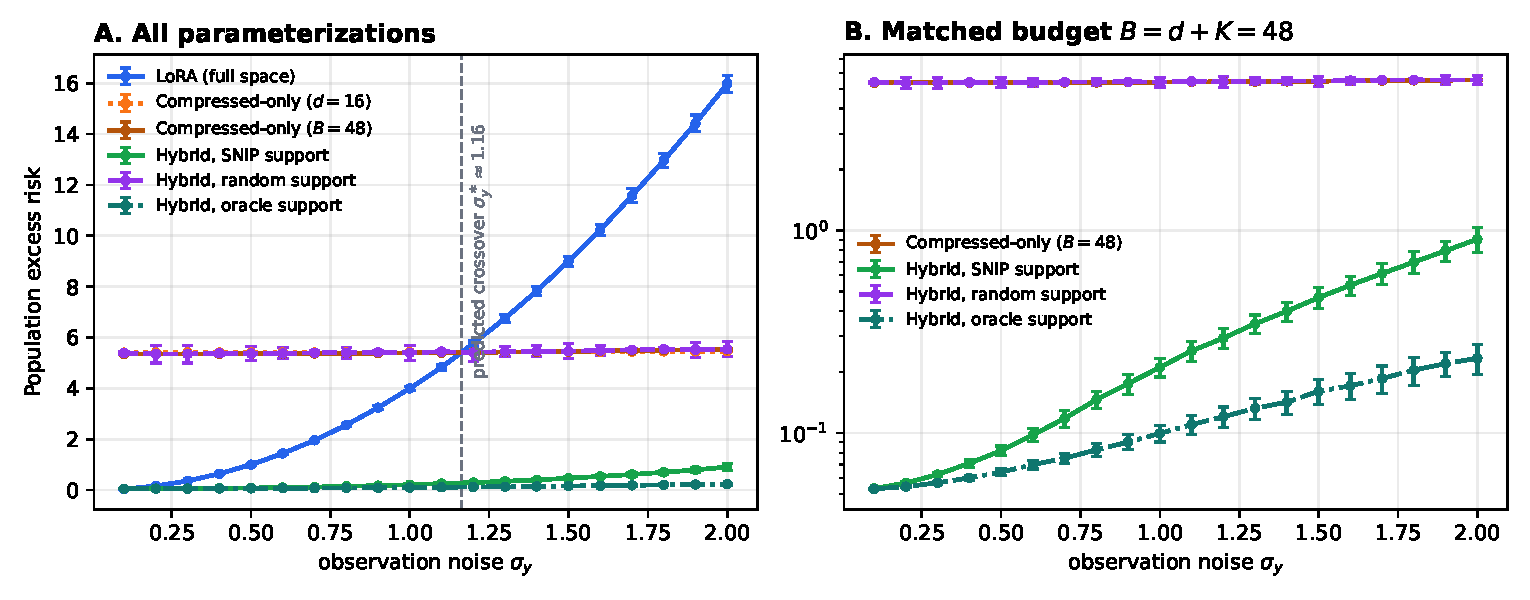
\includegraphics[width=0.9\textwidth]{synthetic_matched_budget.pdf}
    \caption{
    \textbf{Matched-budget comparison in the projection-blind sequence model} ($B=d+K=48$, heavy-tailed target).
    \textbf{A:} population excess risk of all parameterizations; the dashed vertical line marks the fixed-instance full-space/compressed crossover $\sigma_y^\ast\approx 1.16$ predicted by Eq.~\eqref{eq:conditional_compressed_risk}.
    \textbf{B:} matched-budget methods only (log scale). The random-support hybrid nearly coincides with the $B$-dimensional compressed-only estimator on this instance, consistent with the ensemble equality in Corollary~\ref{cor:random_support}; informed supports recover most of the bias, and the gap between the noise-dependent (SNIP-analog) and target-informed top-$K$ supports grows with $\sigma_y$, visualizing the selection-variance effect.
    }
    \label{fig:synthetic_matched_budget}
\end{figure*}

\begin{figure*}[t]
    \centering
    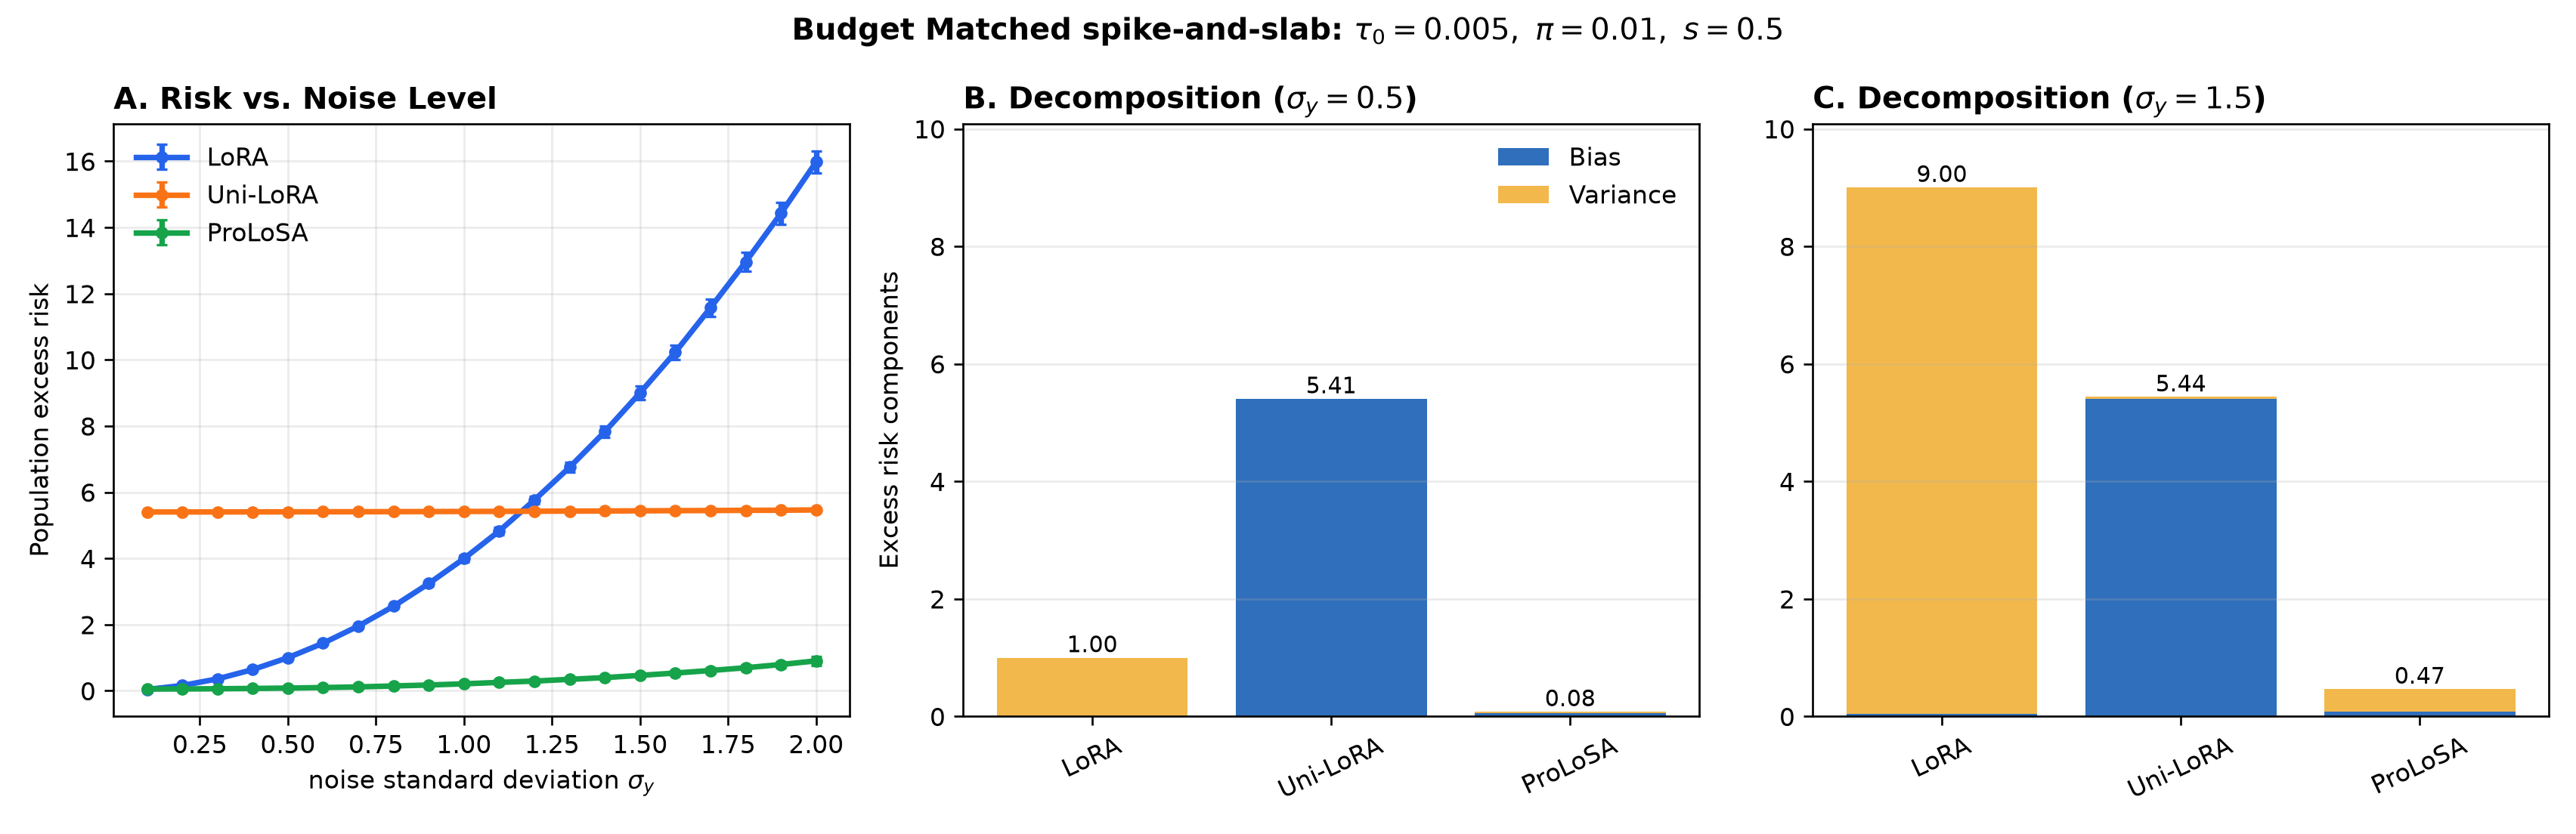
\includegraphics[width=0.65\textwidth]{synthetic_blind_validation.png}
    \caption{
    \textbf{Projection-blind synthetic validation of the compression bias--variance trade-off.}
    One ground-truth update is sampled independently of the projection matrix; both remain fixed across all trials and noise levels. The observation-noise level \(\sigma_y\) controls estimation variance.
    \textbf{A:} population excess risk as \(\sigma_y\) increases; the LoRA/Uni-LoRA crossover at \(\sigma_y\approx 1.16\) matches the conditional form of Proposition~1 in Eq.~\eqref{eq:conditional_compressed_risk}, while ProLoSA retains the variance reduction of compression and corrects most of its bias.
    \textbf{B and C:} empirical bias--variance decompositions at \(\sigma_y=0.5\) and \(\sigma_y=1.5\), respectively.
    }
    \label{fig:synthetic_validation}
\end{figure*}

\subsection{The Bias-Dominated Regime: When Compression Uniformly Fails}
\label{sec:synthetic_failure}

The heavy-tailed mixture above is favorable to sparse correction because its off-subspace residual is concentrated; its modest average energy also lets compression become beneficial once observation noise is sufficiently large.
Proposition~1 predicts that the latter picture reverses when the target becomes dense and high-energy.
To test this failure prediction, we replace the problem-generation law in Eq.~\eqref{eq:synthetic_gt} with
$\Theta_j^\star\sim\mathcal N(0,\tau^2)$, $\tau=0.125$, again draw a single target independently of $P$, and hold it fixed across all observation-noise trials.
The ensemble energy is $v=\tau^2=1.56\times10^{-2}$; for the realized pair $(\theta^\star,P)$, the exact conditional value is
$\hat v_\perp=1.5685\times10^{-2}$.
Both exceed the effective noise $\sigma_y^2/n_{\mathrm{eff}}$ over the entire tested range (at most $7.8\times10^{-3}$ at $\sigma_y=2$), while all remaining settings are unchanged.
This construction models adaptation regimes requiring large, dense parameter changes.

Figure~\ref{fig:synthetic_failure} confirms both parts of the prediction.
First, the risk of Uni-LoRA stays pinned at its fixed-instance projection-bias floor
$\tfrac{1}{2}(D-d)\hat v_\perp=32.0$, which exceeds the risk of full-space LoRA at every tested noise level (LoRA reaches only $16.0$ at $\sigma_y=2$).
Compression is therefore \emph{uniformly} harmful in the tested range, and the conditional crossover
$\sigma_y^\ast=\sqrt{n_{\mathrm{eff}}\hat v_\perp}=2.83$ lies outside it.
Second, ProLoSA no longer helps: with the off-subspace energy spread diffusely over all $D-d$ residual directions, the top-$K$ support carries only $6.9\%$ of the target energy, so the sparse correction recovers only a negligible fraction of the bias and its risk curve nearly coincides with that of Uni-LoRA ($30.4$ vs.\ $32.0$ at $\sigma_y=1.5$)---exactly the unrecoverable case identified in Appendix~\ref{sec:when_fails}.
These results suggest, within a single framework, why compressed LoRA thrives in downstream fine-tuning, whose updates are typically low-energy and approximately sparse (the variance-dominated, recoverable regime), yet is a poor fit for tasks requiring large, dense updates, where any fixed low-dimensional parameterization---with or without sparse correction---is limited.

\begin{figure*}[t]
    \centering
    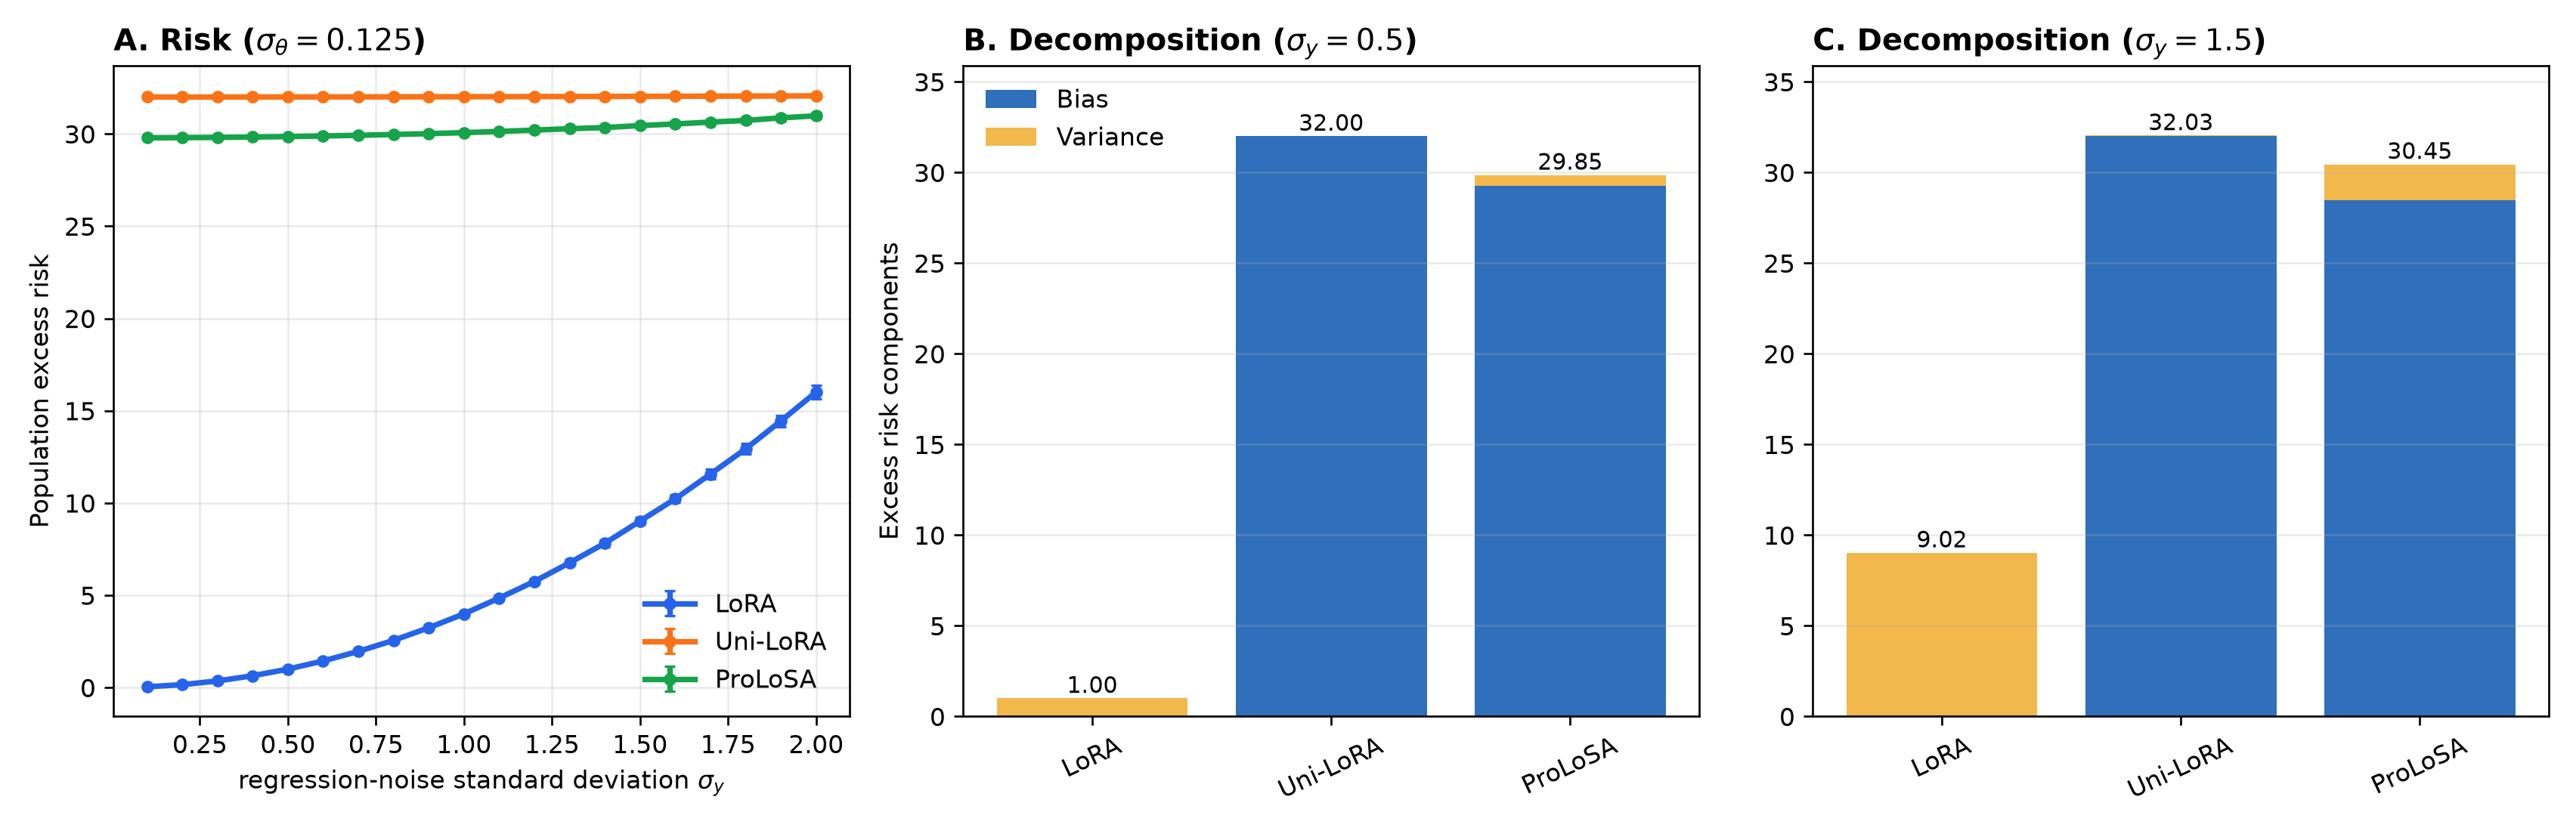
\includegraphics[width=0.65\textwidth]{synthetic_bias_dominated.png}
    \caption{
    \textbf{The bias-dominated failure regime.}
    With a fixed dense Gaussian target ($\tau=0.125$, with realized $\hat v_\perp>\sigma_{\mathrm{eff}}^2$ throughout the tested range), Uni-LoRA is pinned at its bias floor of $32.0$, uniformly worse than LoRA (\textbf{A}), and ProLoSA recovers only a negligible fraction of the diffuse bias (\textbf{B}, \textbf{C}), as predicted by Proposition~1.
    }
    \label{fig:synthetic_failure}
\end{figure*}


\subsection{From the Sequence Model to a Transformer Block}
\label{sec:transformer_synthetic}

The sequence model of Appendices~\ref{sec:synthetic} and~\ref{sec:synthetic_failure} tests the fixed-instance identity in Eq.~\eqref{eq:conditional_compressed_risk}, but deliberately removes several properties of neural
network fine-tuning, including nonlinear parameterization, anisotropic
curvature, finite-step optimization, and data-dependent support selection.
We therefore run a second controlled teacher--student experiment on a single
Transformer block, in which the ground-truth update remains known and its
energy profile controllable. The goal is not the numerical threshold of
Eq.~\eqref{eq:energy_noise_condition}, which is specific to the isotropic
sequence model, but whether the qualitative bias--variance predictions
survive once these idealizations are removed.

\paragraph{Setup.}
We use a standard Transformer block ($d_{\mathrm{model}}=64$, sequence length
$T=32$, $d_{\mathrm{ff}}=256$; multi-head self-attention, a two-layer MLP,
LayerNorm, and residual connections), whose base parameters $W_0$ are
pretrained on a generic synthetic sequence-regression task and then frozen.
We adapt the query and value projections and work directly in the vectorized
\emph{weight-update} space
\begin{equation}
    \theta
    =
    \operatorname{vec}(\Delta W_q,\Delta W_v)
    \in\mathbb{R}^{D},
    \qquad
    D=8192,
\end{equation}
in which the compression $P\theta_d$, the sparse routing, and all energy
measurements are defined; unlike the LoRA factor space, this space is
identifiable (cf.\ the remark after Proposition~\ref{prop:energy_noise}).
The teacher plants a target $\theta^\star$ with one of two energy profiles:
\emph{concentrated} (the sparse heavy-tailed mixture of
Eq.~\eqref{eq:synthetic_gt}) or \emph{diffuse} (dense Gaussian).
Each planted update is then rescaled by a common scalar so that its
functional displacement
\begin{equation}
    \delta_{\mathrm{func}}
    =
    \mathbb{E}_{x}\big[\|f(x;W_0+\Delta W^\star)-f(x;W_0)\|_2^2\big]
    \big/
    \mathbb{E}_{x}\big[\|f(x;W_0)\|_2^2\big]
    \label{eq:functional_displacement}
\end{equation}
equals $10\%$ (concentrated) or $100\%$ (diffuse) of the output variance;
the two profiles thus differ in both magnitude and concentration, mirroring
the ``modest fine-tuning update vs.\ large distribution shift'' contrast of
Appendices~\ref{sec:synthetic}--\ref{sec:synthetic_failure}.
Both targets are almost entirely off-subspace (off-subspace fraction
$\approx 0.99$), but the top-$K$ ($K=64$) coordinates of the residual carry
$99\%$ of its energy in the concentrated profile versus $7\%$ in the diffuse
profile---recoverable versus unrecoverable by construction.
Training data are $y_i=f(x_i;W_0+\Delta W^\star)+\varepsilon_i$ with
$\varepsilon_i\sim\mathcal{N}(0,\sigma_y^2I)$, where $f$ returns the
$d_{\mathrm{model}}$-dimensional pooled hidden representation; the
vector-valued output keeps the planted directions functionally observable.

\paragraph{Compared parameterizations.}
With $W_0$ frozen, every method optimizes its own parameters with AdamW for a
fixed step budget: full fine-tuning of the adapted matrices ($8192$
parameters), rank-$4$ LoRA ($1024$), a matched-budget compressed
parameterization $\theta=P\theta_d$ with $B=d+K=128$, ProLoSA with $d=64$
projected and $K=64$ routed coordinates using the true two-stage warmup SNIP
protocol of Appendix~\ref{sec:routed_sparse_adapter}, a random-support hybrid,
and an oracle-support hybrid.
The saved Transformer implementation defines its target-informed oracle support by
\begin{equation}
 s_i^{\mathrm{oracle}}=\widehat H_{ii}(\theta_i^\star)^2,
 \label{eq:transformer_oracle}
\end{equation}
where $\widehat H$ is a diagonal empirical Gauss--Newton proxy. This is a score on the planted update, not the $H$-projected residual or the exact joint bias reduction. The support is fixed within each teacher grid. The calibration run estimates its own curvature proxy, so its oracle support need not match the noisy grid even when the planted target is unchanged.
We sweep $n\in\{64,\ldots,4096\}$ and $\sigma_y\in\{0.1,\ldots,2.0\}$ with
$M=20$ training-set/optimization seeds per cell. For each profile, the teacher update, pretrained backbone, projections, and noiseless test inputs are fixed before iterating over $n$, noise, and training seed; the full
configuration is given in Appendix~\ref{app:transformer_details}.

\paragraph{Function-space measurement.}
Since parameter-space distances are misleading under nonlinear and
overparameterized parameterizations, we measure excess risk and its
decomposition in function space on a large noiseless test set from the
teacher distribution: with $\bar f(x)=\frac{1}{M}\sum_{m=1}^{M}f_{\hat\theta^{(m)}}(x)$,
\begin{align}
 \mathrm{Bias}_{\mathrm{func}}
 &=\mathbb E_{x,c}\big[(\bar f_c(x)-f_{\theta^\star,c}(x))^2\big],\\
 \mathrm{Variance}_{\mathrm{func}}
 &=\frac1M\sum_{m=1}^M\mathbb E_{x,c}
 \big[(f_{\hat\theta^{(m)},c}(x)-\bar f_c(x))^2\big].
 \label{eq:functional_bias_variance}
\end{align}
Here $\mathbb E_{x,c}$ averages test examples and output coordinates. The stored Transformer metric is excess prediction MSE, without the factor $1/2$ used in the sequence model; its empirical mean equals these two components' sum. Each decomposition is conditional on one teacher and fixed test inputs. We do not pool the two profiles. The 20-seed noisy grid and two-seed noiseless calibration are separate cells, and neither their bias nor their variance is combined. Rechecking the 10,108 saved trials reproduces all 518 cell risk means and standard deviations; every stored function-space bias--variance sum matches its cell mean. The original Transformer Python sources and per-run predictions are not retained in this workspace: fixed-teacher control is supported by saved runner bytecode, logs, and target metadata, but the decomposition cannot be independently recomputed from raw predictions here.

\paragraph{Approximation floors.}
Noiseless large-sample fits confirm that the two constructions instantiate
the intended regimes in function space: the matched-budget compressed
parameterization has an approximation floor of $0.0047$ under the
concentrated target versus $0.041$ under the diffuse target ($\approx 9\times$
larger), and the oracle hybrid removes $99\%$ of the concentrated floor
(to $6\times 10^{-5}$) but only $13\%$ of the diffuse floor (to $0.035$)
(Appendix~\ref{app:transformer_details}).

\paragraph{Results: sample-size crossover and its noise shift.}
Figure~\ref{fig:transformer_risk} shows excess prediction MSE as a
function of $n$.
The qualitative predictions of Appendix~\ref{sec:testable_predictions} hold in
both regimes: at small $n$, full-space methods are variance-dominated and the
compressed parameterization wins by up to an order of magnitude; as $n$
grows, LoRA crosses below the compressed baseline---at
$n\approx 2^9$--$2^{10}$ for the diffuse target and
$n\approx 2^{11}$ for the concentrated target at $\sigma_y=0.5$---and the
crossover point moves to larger $n$ as the label noise increases (at
$\sigma_y=2$ it exceeds $n=10^3$ in both regimes), exactly the
$n^\star\propto A_{\mathrm{var}}/B_{\mathrm{proj}}$ shift predicted by
Eq.~\eqref{eq:risk_gap_n}.

\paragraph{Results: decomposition, recoverability, and matched budgets.}
Figure~\ref{fig:transformer_biasvar} reports the function-space
decomposition of Eq.~\eqref{eq:functional_bias_variance}.
At $n=64$ the excess risk of LoRA is almost entirely variance, which every
compressed parameterization suppresses by an order of magnitude; at $n=4096$
the compressed methods are pinned at their bias floors while LoRA's bias is
far smaller---the predicted reversal of the bias and variance orderings.
Sparse residual correction behaves exactly as the recoverability analysis
predicts: under the concentrated target, ProLoSA reduces the compressed bias
floor by roughly half (excess risk $0.0030$ vs.\ $0.0052$ at $n=4096$,
$\sigma_y=1$) with the oracle support reaching $5.6\times 10^{-4}$, whereas
under the diffuse target even the oracle support barely helps
($0.0356$ vs.\ $0.0412$), so the limitation is the energy profile itself,
not support selection.
The matched-budget prediction also carries over: the random-support hybrid
never beats the compressed baseline of the same budget, tying it under the
concentrated target ($0.0053$ vs.\ $0.0052$) and running slightly worse under
the diffuse target ($0.0439$ vs.\ $0.0412$)---a deviation from the exact
isotropic tie of Corollary~\ref{cor:random_support} that is consistent with
anisotropic curvature.
Finally, the experiment also exposes the predicted cost of data-dependent
selection: in the small-$n$, high-noise corner of the concentrated regime
(e.g., $n=64$, $\sigma_y=1.5$), ProLoSA's noisy warmup scores select
unreliable supports and it falls behind the compressed baseline
($0.105$ vs.\ $0.066$), the selection-variance effect anticipated in the
remark after Proposition~\ref{prop:matched_budget}.
In sum, all four qualitative predictions persist under nonlinear
parameterization, anisotropic curvature, finite-step optimization, and
data-dependent support selection, and the observed deviations occur precisely
where the theory's idealizations are known to break.

\begin{figure*}[t]
    \centering
    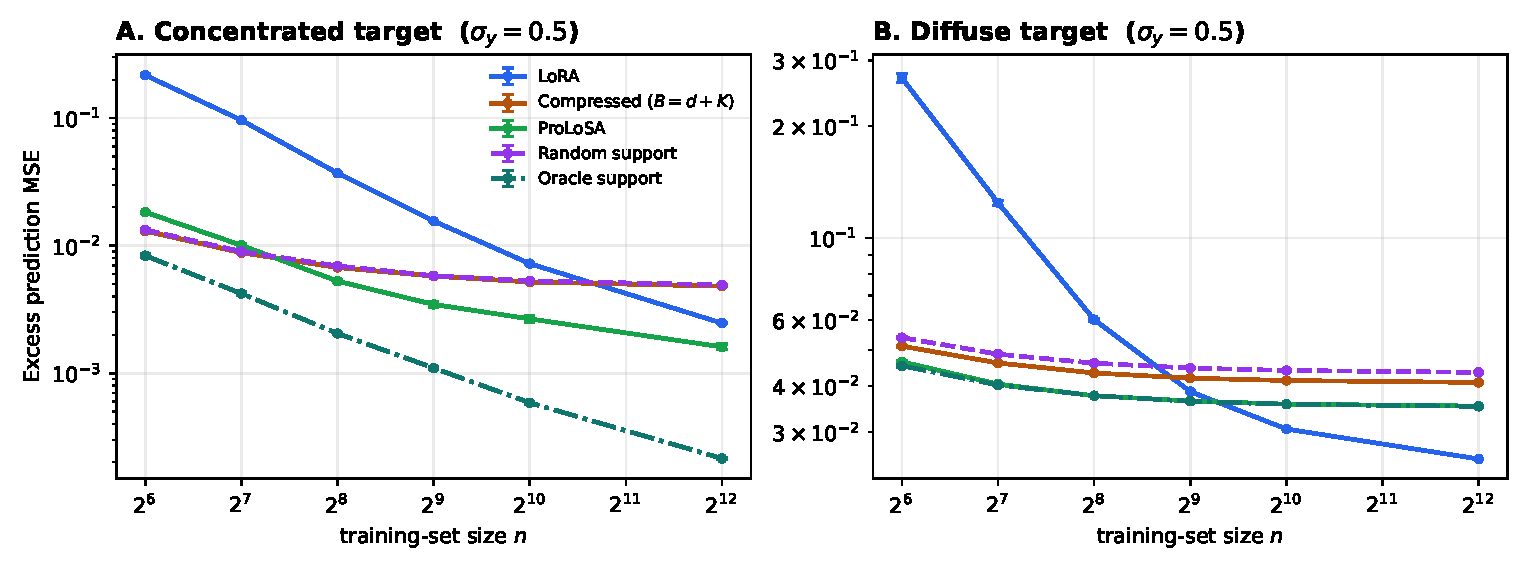
\includegraphics[width=0.95\textwidth]{transformer_risk_vs_n.pdf}
    \caption{
    \textbf{Transformer teacher--student: excess prediction MSE vs.\ $n$}
    ($\sigma_y=0.5$; mean $\pm$ s.e.\ over $20$ seeds; log--log scale).
    LoRA crosses below the matched-budget compressed baseline as $n$ grows in
    both regimes; ProLoSA improves on the compressed baseline under the
    concentrated target, where the random-support hybrid merely tracks it,
    while under the diffuse target ProLoSA nearly coincides with the oracle,
    which itself recovers little of the bias floor.
    }
    \label{fig:transformer_risk}
\end{figure*}

\begin{figure*}[t]
    \centering
    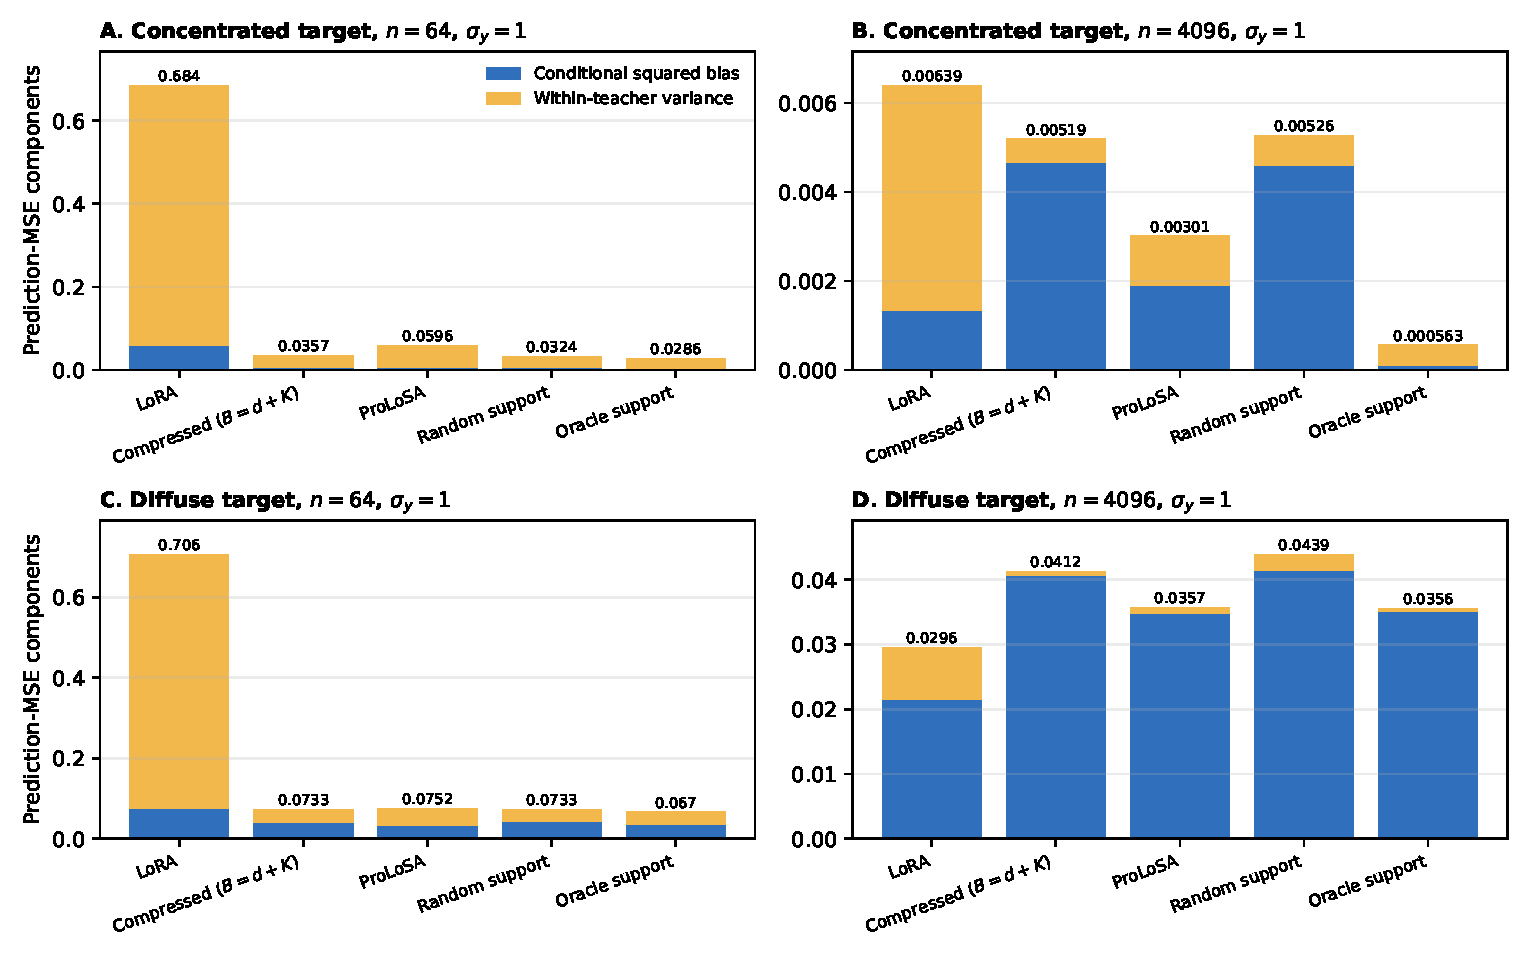
\includegraphics[width=0.9\textwidth]{transformer_biasvar.pdf}
    \caption{
    \textbf{Transformer teacher--student: function-space bias--variance
    decomposition} (Eq.~\eqref{eq:functional_bias_variance}, $\sigma_y=1$).
    Left column ($n=64$): variance dominates and compression removes it.
    Right column ($n=4096$): compressed parameterizations are pinned at their
    bias floors; sparse correction recovers a large fraction of the
    concentrated floor (top) but almost none of the diffuse floor (bottom),
    where even the oracle support fails, and the random-support hybrid does
    not improve on matched-budget compression.
    }
    \label{fig:transformer_biasvar}
\end{figure*}


\subsection{Testing the Downstream Predictions on Real Fine-Tuning}
\label{sec:real_model_validation}

The synthetic experiments establish the predicted mechanism under controlled assumptions.
We next examine three of its signatures in RoBERTa-large fine-tuning: the $1/n$ dependence of the compression advantage (E1), the bias--variance decomposition itself (E3), and the sparse recoverability of off-subspace residuals (E5).
Uni-LoRA and ProLoSA use matched compressed-parameter budgets, while rank-$4$ LoRA serves as the full-space baseline; all configurations follow Appendix Table~\ref{tab:glue_hyperparams}, and comparisons within each experiment share data subsets and evaluation sets.
Because Eq.~\eqref{eq:compressed_excess_risk} concerns predictive risk rather than raw parameter distance, E1 uses dev loss and E3 uses predictive probabilities as their primary observables.
For E5, we approximate the local curvature by the diagonal empirical Fisher,
$\hat H_{ii}=B^{-1}\sum_b(\partial\ell_b/\partial\theta_i)^2$, and weight residual coordinates after specifying the projection metric explicitly.

\begin{table*}[t]
\centering
\small
\caption{Real-model tests of the theoretical mechanism. E1 probes the sample-size signature in Eq.~\eqref{eq:risk_gap_n}; E3 decomposes predictive variability and a reference-based bias proxy; E5 diagnoses coordinate concentration related to the recoverability condition underlying Proposition~\ref{prop:matched_budget}.}
\label{tab:pred_overview}
\resizebox{\linewidth}{!}{%
\begin{tabular}{llll}
\toprule
Exp. & Theoretical target & Primary observable & Expected signature \\
\midrule
E1 & P1: sample-size scaling & $\Delta L_{\mathrm{dev}}(n)$ & positive $1/n$ component \\
E3 & bias--variance mechanism & $V_{\mathrm{stat}}$, $V_{\mathrm{opt}}$, $\mathrm{Bias}^2$ & compression lowers variance but raises bias \\
E5 & P4: sparse recoverability & Fisher-weighted residual capture & SNIP enrichment over random support \\
\bottomrule
\end{tabular}}
\end{table*}

\paragraph{E1: sample-size scaling (P1).}
We use fixed stratified subsets of fractions $p\in\{1\%,2\%,5\%,10\%,25\%,50\%,100\%\}$ on SST-2/QNLI and $p\in\{25\%,50\%,100\%\}$ on CoLA/MRPC. Each fraction uses subset seed 12345 for all methods and training seeds $s=0,\ldots,4$, with a fixed full-data update-step budget. For each run, dev loss is the minimum over its evaluation checkpoints, rather than a population-risk observation. We retain the dedicated-adapter-learning-rate LoRA reruns on SST-2/CoLA and the existing LoRA runs on QNLI/MRPC.
Define $\delta_s(p)=L_{L,s}(p)-L_{U,s}(p)$. We compute the mean and pointwise 95\% interval as
\begin{equation}
 \bar\delta(p)\ \pm\ t_{4,0.975}\,s_\delta(p)/\sqrt{5},
 \qquad s_\delta^2(p)=\tfrac14\sum_{s=0}^4(\delta_s(p)-\bar\delta(p))^2.
\end{equation}
The intervals in Table~\ref{tab:e1_paired_ci} use the paired differences themselves. They are conditional on the fixed subsets and dev set, reflect training randomness (including projection initialization), and are neither simultaneous intervals nor estimates of population sampling uncertainty.

We fit the same paired means to $a/n-b$ by unweighted least squares using actual subset sizes, both freely and with $a,b\geq0$ (Table~\ref{tab:e1_paired_fit}). All $5^5=3125$ ordered bootstrap resamples of complete seed trajectories give descriptive percentile intervals for both coefficients, retaining dependence across fractions. With only five trajectories, especially at a constraint boundary, these intervals are limited sensitivity estimates. Point residuals and bootstrap intervals for residual RMSE are retained in the reanalysis artifact.
SST-2's free fit has $\hat a=52.14$, $\hat b=-0.0171$, $R^2=0.485$, while CoLA's mean fit has $R^2=0.014$ on the same paired-mean scale. QNLI has $\hat a=-43.90$ with a bootstrap interval wholly below zero; imposing the theoretical signs gives $R^2=-0.363$. All four constrained point fits put $b$ at zero, so none yields a finite positive crossover. Negative slopes, structured residuals, and positive free intercepts indicate mismatch with the local asymptotic model under this protocol; an insufficient range of sample sizes alone does not explain them.

\begin{table*}[t]
\centering
\scriptsize
\setlength{\tabcolsep}{3pt}
\caption{\textbf{E1: sample-size scaling.} RoBERTa-large dev loss (mean$_{\pm\mathrm{std}}$ over 5 seeds). $\Delta=L_{\mathrm{dev}}^{\mathrm{LoRA}}-L_{\mathrm{dev}}^{\text{Uni-LoRA}}$; positive values favor compression.}
\label{tab:e1_crossover}
\begin{tabular}{lcccccccc}
\toprule
& \multicolumn{4}{c}{SST-2} & \multicolumn{4}{c}{QNLI} \\
\cmidrule(lr){2-5}\cmidrule(lr){6-9}
$p$ & LoRA & Uni-LoRA & ProLoSA & $\Delta(p)$ & LoRA & Uni-LoRA & ProLoSA & $\Delta(p)$ \\
\midrule
$1\%$   & $.445_{\pm.035}$ & $.378_{\pm.048}$ & $.382_{\pm.081}$ & $.067$  & $.710_{\pm.038}$ & $.750_{\pm.034}$ & $.765_{\pm.058}$ & $-.040$ \\
$2\%$   & $.361_{\pm.053}$ & $.263_{\pm.028}$ & $.314_{\pm.023}$ & $.098$  & $.559_{\pm.078}$ & $.482_{\pm.045}$ & $.564_{\pm.071}$ & $.078$ \\
$5\%$   & $.256_{\pm.054}$ & $.183_{\pm.030}$ & $.188_{\pm.011}$ & $.073$  & $.407_{\pm.059}$ & $.259_{\pm.022}$ & $.289_{\pm.031}$ & $.147$ \\
$10\%$  & $.178_{\pm.009}$ & $.156_{\pm.009}$ & $.155_{\pm.022}$ & $.023$  & $.250_{\pm.024}$ & $.225_{\pm.009}$ & $.212_{\pm.005}$ & $.025$ \\
$25\%$  & $.139_{\pm.011}$ & $.139_{\pm.010}$ & $.139_{\pm.010}$ & $-.000$ & $.192_{\pm.016}$ & $.179_{\pm.004}$ & $.179_{\pm.006}$ & $.013$ \\
$50\%$  & $.133_{\pm.006}$ & $.132_{\pm.005}$ & $.132_{\pm.006}$ & $.002$  & $.168_{\pm.005}$ & $.158_{\pm.002}$ & $.158_{\pm.002}$ & $.010$ \\
$100\%$ & $.127_{\pm.006}$ & $.125_{\pm.006}$ & $.127_{\pm.005}$ & $.002$  & $.160_{\pm.007}$ & $.148_{\pm.004}$ & $.148_{\pm.003}$ & $.012$ \\
\bottomrule
\end{tabular}
\end{table*}

\begin{table*}[t]
\centering\small
\caption{Paired E1 mean loss gaps and pointwise 95\% Student-$t$ intervals (five training seeds, four degrees of freedom). The training subset is fixed at each fraction; these intervals do not measure uncertainty over new training sets or new dev sets.}
\label{tab:e1_paired_ci}
\begin{tabular}{lrrrr}
\toprule
Task & Fraction & $n$ & Mean gap & 95\% interval \\
\midrule
SST-2 & 1\% & 673 & 0.0671 & [-0.0206, 0.1549] \\
SST-2 & 2\% & 1346 & 0.0975 & [0.0395, 0.1556] \\
SST-2 & 5\% & 3367 & 0.0735 & [-0.0177, 0.1647] \\
SST-2 & 10\% & 6734 & 0.0227 & [0.0077, 0.0377] \\
SST-2 & 25\% & 16837 & -0.0002 & [-0.0200, 0.0196] \\
SST-2 & 50\% & 33674 & 0.0018 & [-0.0106, 0.0143] \\
SST-2 & 100\% & 67349 & 0.0023 & [-0.0083, 0.0129] \\
QNLI & 1\% & 1047 & -0.0395 & [-0.0736, -0.0054] \\
QNLI & 2\% & 2094 & 0.0776 & [-0.0159, 0.1710] \\
QNLI & 5\% & 5237 & 0.1474 & [0.0548, 0.2400] \\
QNLI & 10\% & 10474 & 0.0250 & [-0.0006, 0.0507] \\
QNLI & 25\% & 26185 & 0.0131 & [-0.0074, 0.0335] \\
QNLI & 50\% & 52371 & 0.0102 & [0.0053, 0.0151] \\
QNLI & 100\% & 104743 & 0.0125 & [0.0075, 0.0175] \\
CoLA & 25\% & 2137 & 0.0362 & [-0.0794, 0.1517] \\
CoLA & 50\% & 4275 & 0.0669 & [-0.0158, 0.1497] \\
CoLA & 100\% & 8551 & 0.0224 & [-0.0083, 0.0531] \\
MRPC & 25\% & 917 & -0.0003 & [-0.1204, 0.1197] \\
MRPC & 50\% & 1834 & 0.0009 & [-0.0208, 0.0226] \\
MRPC & 100\% & 3668 & 0.0156 & [0.0008, 0.0303] \\
\bottomrule
\end{tabular}
\end{table*}

\begin{table*}[t]
\centering\scriptsize
\caption{Unweighted fits of paired mean gaps to $a/n-b$. Brackets are descriptive 95\% percentile intervals from all $5^5=3125$ resamples of complete seed trajectories. Constrained fits impose $a,b\geq0$; boundary intervals such as $[0,0]$ are a consequence of the constraint and the five observed seeds.}
\label{tab:e1_paired_fit}
\begin{tabular}{llrrrr}
\toprule
Task & Fit & $a$ [interval] & $b$ [interval] & RMSE & $R^2$ \\
\midrule
SST-2 & Free & 52.14 [11.02, 86.04] & -0.0171 [-0.0344, -0.0020] & 0.0270 & 0.485 \\
SST-2 & Constrained & 68.69 [36.95, 98.78] & 0.0000 [0.0000, 0.0000] & 0.0302 & 0.358 \\
QNLI & Free & -43.90 [-63.14, -29.14] & -0.0464 [-0.0618, -0.0356] & 0.0538 & 0.065 \\
QNLI & Constrained & 25.83 [0.00, 57.84] & 0.0000 [0.0000, 0.0000] & 0.0650 & -0.363 \\
CoLA & Free & 14.83 [-218.67, 278.07] & -0.0378 [-0.0910, 0.0229] & 0.0185 & 0.014 \\
CoLA & Constrained & 122.47 [0.00, 278.07] & 0.0000 [0.0000, 0.0229] & 0.0257 & -0.902 \\
MRPC & Free & -17.00 [-119.24, 85.23] & -0.0162 [-0.0564, 0.0240] & 0.0043 & 0.641 \\
MRPC & Constrained & 2.81 [0.00, 85.23] & 0.0000 [0.0000, 0.0278] & 0.0088 & -0.477 \\
\bottomrule
\end{tabular}
\end{table*}


\paragraph{E3: empirical bias--variance decomposition (mechanism).}
We use five independently drawn 80\% stratified subsets of the available training corpus (without replacement within a subset; subset seeds 101--105) and two training seeds (0, 1) per subset. The dev examples and their ordering remain fixed. Let $f_{bs}$ be the predictive-probability vector, $\bar f_b$ its seed mean, and $\bar f$ the grand mean. Write $\|u\|_N^2=N^{-1}\sum_{i,c}u_{ic}^2$ to average over examples and sum over classes. For $B=5,S=2$, the reported finite-replicate convention is
\begin{align}
 \widehat V_{\rm opt}&=\frac{1}{B(S-1)}\sum_{b,s}\|f_{bs}-\bar f_b\|_N^2,\\
 \widehat V_{\rm between}&=\frac{1}{B-1}\sum_b\|\bar f_b-\bar f\|_N^2,\qquad
 \widehat V_{\rm stat}=\max\{\widehat V_{\rm between}-\widehat V_{\rm opt}/S,0\}.
\end{align}
The subtraction removes within-subset variability leaking into the subset means under a nested replicate model. The same seed labels recur across subsets; a crossed data/seed sensitivity calculation, subtracting the estimated data--seed interaction divided by $S$ instead, gives signed data components $(0.00301,0.00057,0.00656)$ on CoLA and $(0.00890,0.00157,-0.00110)$ on MRPC (LoRA, Uni-LoRA, ProLoSA). The nested convention gives $-0.00115$ for MRPC ProLoSA before clipping; the displayed zero is not evidence that its statistical variance vanishes. Two seed levels make either variance-component estimate imprecise. Moreover, these are resampling diagnostics conditional on the observed corpus, not an independent-population estimate of the $1/n$ coefficient.
Within-subset variability includes initialization, minibatch order, optimization, and the projection seed, which defaults to the training seed. We retain the historical $V_{\rm opt}$ notation but label this full component as training-seed variance in the figure.

The reference $f^{\rm ref}$ averages eight full-data LoRA predictions per task: three rank-4 E4 runs and five retained rank-64 E3 reference runs. The original quality rule retains rank-64 references with dev score at least 85\% of the best reference score; it excludes five failed CoLA runs and no MRPC runs. This is dev-based reference selection. Squared bias is the plug-in proxy $\|\bar f-f^{\rm ref}\|_N^2$; finite-ensemble noise and dev selection remain, so its sum with corrected variance is not an unbiased risk estimate or an exact empirical decomposition.

On CoLA, $87.8\%$ of the LoRA-to-Uni-LoRA variance reduction is attributable to training seeds. On MRPC, ProLoSA lowers the bias proxy and total variance relative to Uni-LoRA; CoLA lacks this bias correction. Table~\ref{tab:e3_reference} replaces the reference by the rank-4-only and rank-64-only ensembles and all eight leave-one-reference-out ensembles. The complete bias ordering remains LoRA $<$ Uni-LoRA $<$ ProLoSA on CoLA and LoRA $<$ ProLoSA $<$ Uni-LoRA on MRPC in every case. This robustness concerns ordering, not identification of population bias.

\begin{table*}[t]
\centering
\small
\setlength{\tabcolsep}{5pt}
\caption{\textbf{E3: empirical bias--variance decomposition in predictive-probability space.} Values are per-example averages over five data resamples and two optimization seeds. $V_{\mathrm{stat}}$ is finite-replicate corrected, $V_{\mathrm{total}}=V_{\mathrm{opt}}+V_{\mathrm{stat}}$, and Total is the descriptive sum $\mathrm{Bias}^2+V_{\mathrm{total}}$. The zero data component for MRPC ProLoSA is clipped.}
\label{tab:e3_decomp}
\begin{tabular}{llccccc}
\toprule
Task & Method & $V_{\mathrm{opt}}$ & $V_{\mathrm{stat}}$ & $V_{\mathrm{total}}$ & $\mathrm{Bias}^2$ & Total \\
\midrule
CoLA & LoRA     & $.0593$ & $.0043$ & $.0636$ & $.0136$ & $.0772$ \\
     & Uni-LoRA & $.0326$ & $.0006$ & $.0332$ & $.0309$ & $\mathbf{.0641}$ \\
     & ProLoSA  & $.0306$ & $.0063$ & $.0369$ & $.0319$ & $.0688$ \\
\midrule
MRPC & LoRA     & $.0283$ & $.0091$ & $.0374$ & $.0124$ & $.0498$ \\
     & Uni-LoRA & $.0313$ & $.0013$ & $.0326$ & $.0219$ & $.0545$ \\
     & ProLoSA  & $.0303$ & $.0000$ & $.0303$ & $.0180$ & $\mathbf{.0483}$ \\
\bottomrule
\end{tabular}
\end{table*}

\begin{table*}[t]
\centering\small
\caption{Sensitivity of squared bias proxies to the full-data reference: mixed (3 rank-4 + 5 rank-64 runs), rank-4 only, rank-64 only, and the range over eight leave-one-reference-out ensembles. Ranges are sensitivity checks, not confidence intervals.}
\label{tab:e3_reference}
\begin{tabular}{llrrrr}
\toprule
Task & Method & Mixed & Rank 4 & Rank 64 & Leave-one-out range \\
\midrule
CoLA & LoRA & 0.01363 & 0.02275 & 0.01769 & [0.01328, 0.01523] \\
CoLA & Uni-LoRA & 0.03091 & 0.03195 & 0.03982 & [0.02972, 0.03503] \\
CoLA & ProLoSA & 0.03189 & 0.03440 & 0.03990 & [0.03081, 0.03594] \\
MRPC & LoRA & 0.01236 & 0.02146 & 0.01703 & [0.01184, 0.01426] \\
MRPC & Uni-LoRA & 0.02187 & 0.03247 & 0.02563 & [0.02103, 0.02418] \\
MRPC & ProLoSA & 0.01804 & 0.02927 & 0.02142 & [0.01762, 0.02003] \\
\bottomrule
\end{tabular}
\end{table*}


\paragraph{E5: residual geometry and coordinate-support reference (P4).}
We reanalyse the saved artifacts without retraining, explicitly averaging only full-data rank-4 LoRA targets: eight runs each on CoLA/MRPC and five each on QNLI/RTE/STS-B. Dedicated-learning-rate reruns replace superseded runs. We use the full-data seed-0 ProLoSA support in each task, chosen by this fixed provenance rule, rather than selecting the support with highest capture. All $D=1{,}769{,}472$ factor coordinates are candidate support positions; the stored offsets form a bijection to this ordering. CoLA/MRPC use $(d,K)=(14400,8640)$; the other tasks use $(22320,721)$ (the saved mask has 721 active entries although its nominal budget is 720). These are single-support diagnostics, not averages across support seeds or the MRPC configuration of E3. All reported energy fractions use this explicit full-data target/support selection.

Let $\bar\theta_L$ denote this mean factor-space target proxy. The original coordinate diagnostic forms the Euclidean residual
$q_E=(I-PP^\top)\bar\theta_L$ and then weights its coordinates by $\hat H_{ii}$.
The saved $\hat H$ averages squared minibatch-mean loss gradients over up to 200 training batches of size 16 (156 batches for RTE) at one full-data LoRA checkpoint per task. It is a diagonal sensitivity proxy, not an exact Hessian or the per-example Fisher. Factor coordinates and their cross-seed mean are gauge-dependent, which further limits identification with functional projection bias.
The metric projection instead gives
\begin{equation}
 q_H=\bar\theta_L-P(P^\top\hat H P)^\dagger P^\top\hat H\bar\theta_L.
\end{equation}
For one-hot sharing, $q_E$ subtracts the ordinary mean within each bucket, whereas $q_H$ subtracts its $\hat H$-weighted mean. Hence post-weighting an Euclidean residual does not compute an $H$-orthogonal residual.

For either fixed residual $q$, let $e_i=\hat H_{ii}q_i^2$ and $\rho_{I,H}^2=\sum_{i\in I}e_i/\sum_i e_i$. Uniform sampling of $K$ coordinates without replacement gives
\begin{equation}
 \mathbb E_I[\rho_{I,H}^2]
 =\frac{\sum_i\Pr(i\in I)e_i}{\sum_i e_i}=\frac KD.
\end{equation}
More generally, a candidate set $C$ gives $(K/|C|)\sum_{i\in C}e_i/\sum_i e_i$; residual-subspace dimension $D-d$ is not the number of original-coordinate candidates. Enrichment in Table~\ref{tab:e5_recoverability} therefore uses $K/D$. Table~\ref{tab:e5_random} directly checks this reference with 10,000 uniform supports per task. The sample means agree with $K/D$ within two Monte Carlo standard errors; the broad, asymmetric support distribution is reported separately from uncertainty in its mean.

Coordinate capture still differs from joint approximation-bias recovery, even on $q_H$. To measure the latter under the same diagonal proxy, we refit bucket means on the unselected coordinates and fit selected coordinates freely, computing
\begin{equation}
 \gamma_{I,H}=1-
 \frac{\min_{z,\alpha}\|\bar\theta_L-Pz-E_I\alpha\|_{\hat H}^2}
 {\|q_H\|_{\hat H}^2}.
\end{equation}
On MRPC, the $q_E$ coordinate fraction is $18.04\%$, the $q_H$ coordinate fraction is $2.67\%$, and $\gamma_{I,H}=5.68\%$ (Table~\ref{tab:e5_geometry}). The gap across these quantities is substantial. The latter holds $d$ fixed and is not the matched-budget benefit relative to a larger compressed space; it also omits training and support-selection noise. The observed coordinate enrichment supports a sensitivity diagnostic, not a direct verification of the population-energy condition in Proposition~\ref{prop:matched_budget}. Unweighted coordinate enrichment remains below one on all five tasks.

\begin{table*}[t]
\centering\small
\caption{E5 coordinate-energy diagnostics on an explicitly full-data LoRA target proxy. $q_E=(I-PP^\top)\Delta\theta$; oracle and SNIP capture fractions of $\sum_i\hat H_{ii}q_{E,i}^2$. The uniform-coordinate reference is $K/D$, $D=1{,}769{,}472$.}
\label{tab:e5_recoverability}
\begin{tabular}{lrrrrr}
\toprule
Task & $K$ & Oracle & SNIP & $K/D$ & Enrichment \\
\midrule
CoLA & 8640 & 0.4987 & 0.0791 & 0.004883 & $16.21\times$ \\
MRPC & 8640 & 0.6945 & 0.1804 & 0.004883 & $36.94\times$ \\
QNLI & 721 & 0.1446 & 0.0312 & 0.000407 & $76.52\times$ \\
RTE & 721 & 0.3374 & 0.0114 & 0.000407 & $27.98\times$ \\
STS-B & 721 & 0.5191 & 0.0791 & 0.000407 & $194.13\times$ \\
\bottomrule
\end{tabular}
\end{table*}

\begin{table*}[t]
\centering\scriptsize
\caption{Effect of projection geometry with the same target, Fisher diagonal, and saved SNIP support. Coordinate capture on $q_E$ and $q_H$ uses each residual's own total weighted energy. Joint recovery refits the compressed and sparse coefficients under the diagonal metric and is normalized by $\|q_H\|_{\hat H}^2$.}
\label{tab:e5_geometry}
\begin{tabular}{lrrrr}
\toprule
Task & Capture on $q_E$ & Capture on $q_H$ & Joint recovery & $\|q_H\|_{\hat H}^2/\|q_E\|_{\hat H}^2$ \\
\midrule
CoLA & 7.915\% & 1.188\% & 2.347\% & 0.767 \\
MRPC & 18.037\% & 2.667\% & 5.683\% & 0.567 \\
QNLI & 3.118\% & 0.138\% & 0.384\% & 0.836 \\
RTE & 1.140\% & 0.078\% & 0.239\% & 0.590 \\
STS-B & 7.910\% & 0.198\% & 0.874\% & 0.471 \\
\bottomrule
\end{tabular}
\end{table*}

\begin{table*}[t]
\centering\small
\caption{Uniform random-support check: 10,000 independent size-$K$ subsets drawn without replacement from all $D$ original coordinates (values in percent). The central 95\% range describes random-support variation; it is not an interval for the mean. The last column counts draws reaching the observed SNIP capture on $q_E$.}
\label{tab:e5_random}
\begin{tabular}{lrrrr}
\toprule
Task & Exact mean & Sample mean & Central 95\% range & Exceedances \\
\midrule
CoLA & 0.4883 & 0.4875 & [0.3639, 0.8057] & 0 \\
MRPC & 0.4883 & 0.4889 & [0.2586, 1.3675] & 0 \\
QNLI & 0.0407 & 0.0407 & [0.0259, 0.0838] & 0 \\
RTE & 0.0407 & 0.0402 & [0.0150, 0.1289] & 8 \\
STS-B & 0.0407 & 0.0420 & [0.0102, 0.1840] & 0 \\
\bottomrule
\end{tabular}
\end{table*}



\subsection{Synthetic Experiment Configuration}

Table~\ref{tab:synthetic_hyperparams} summarizes the configuration used for the projection-blind synthetic validation experiment in Appendix~\ref{sec:synthetic} and the bias-dominated failure experiment in Appendix~\ref{sec:synthetic_failure}.
The matched-budget comparison of Figure~\ref{fig:synthetic_matched_budget} reuses the identical target, projection, and per-trial noise realizations (same master seed), and adds a compressed-only estimator with a $B=48$-dimensional projection of the same construction, a hybrid with a uniformly random size-$32$ support redrawn per trial, and a hybrid with the oracle support given by the top-$32$ coordinates of the true off-subspace residual $(I-PP^\top)\theta^\star$.

\begin{table}[htbp]
\centering
\small
\begin{tabular}{lc}
\toprule
Hyperparameter & Value \\
\midrule
Full dimension \(D\) & 4096 \\
Compressed dimension \(d\) & 16 \\
Sparse budget \(K\) & 32 \\
Ground-truth prior (main) & sparse heavy-tailed mixture, Eq.~\eqref{eq:synthetic_gt} \\
Mixture sparsity \(\pi\) & 0.01 \\
Gaussian std.\ \(\tau_0\) & 0.005 \\
Student-\(t\) d.o.f.\ \(\nu\) / std.\ \(\tau_1\) & 3 / 0.5 \\
Ground-truth prior (failure regime) & dense Gaussian \(\mathcal{N}(0,\tau^2)\), \(\tau=0.125\) (Sec.~\ref{sec:synthetic_failure}) \\
Effective sample size \(n_{\mathrm{eff}}\) & 512 \\
Noise std.\ \(\sigma_y\) & grid over \([0.1, 2.0]\) \\
Number of trials \(M\) & 200 \\
Projection type & random orthonormal (QR of a Gaussian matrix) \\
Sparse support & top-\(K\) of post-warmup residual \(|y-PP^\top y|\) \\
Evaluation metric & population excess risk \\
Random seed & 13 \\
\bottomrule
\end{tabular}
\caption{Configuration of the projection-blind synthetic bias--variance validation and failure-regime experiments. For each regime, the target and column-orthonormal projection are drawn independently once and then fixed across all noise trials. Under the isotropic analysis of Appendix~\ref{app:energy_noise_condition}, the random orthonormal projection is exchangeable in expectation with the normalized one-hot construction used in the real-model experiments.}
\label{tab:synthetic_hyperparams}
\end{table}

\subsection{Transformer Teacher--Student Configuration}
\label{app:transformer_details}

Table~\ref{tab:transformer_hyperparams} lists the full configuration of the
Transformer teacher--student experiment of Appendix~\ref{sec:transformer_synthetic}.
The base parameters $W_0$ are pretrained once on a generic synthetic
sequence-regression task and shared by all methods, target profiles, and grid
cells; the teacher, planted update, projection, and training seeds are
controlled by separate deterministic seeds.
The concentrated and diffuse targets are planted directly in the vectorized
weight-update space $\operatorname{vec}(\Delta W_q,\Delta W_v)$ and rescaled
to the functional displacements in the table; the realized off-subspace
fractions are $0.991$ (concentrated) and $0.994$ (diffuse), with top-$K$
residual energy fractions of $0.988$ and $0.068$, respectively.

\begin{table}[htbp]
\centering
\small
\begin{tabular}{@{}p{0.35\linewidth}p{0.60\linewidth}@{}}
\toprule
Hyperparameter & Value \\
\midrule
Block & $d_{\mathrm{model}}=64$, $T=32$, $d_{\mathrm{ff}}=256$ \\
Adapted modules & $W_q$, $W_v$ \\
Update-space dimension $D$ & 8192 \\
LoRA rank & 4 (1024 trainable parameters) \\
Compressed budget $B=d+K$ & $128$ ($d=64$, $K=64$) \\
Target profiles & spike--slab ($\pi=0.01$, $\tau_0=0.005$, $t_3$ slab, std $0.5$); dense Gaussian \\
Functional displacement $\delta_{\mathrm{func}}$ & $10\%$ (concentrated) / $100\%$ (diffuse) \\
Optimizer & AdamW, lr $5\times10^{-3}$, $1000$ steps, batch size $128$, grad.\ clip $1.0$ \\
ProLoSA warmup / SNIP window & $10\%$ / $128$ steps \\
Grid & $n\in\{64,128,256,512,1024,4096\}$, $\sigma_y\in\{0.1,0.25,0.5,1,1.5,2\}$ \\
Seeds per cell & 20 (independent training sets and optimization seeds) \\
Evaluation & prediction MSE on $1024$ fixed noiseless teacher samples \\
Oracle support & top-$K$ of $\widehat H_{ii}(\theta_i^\star)^2$, diagonal empirical Gauss--Newton proxy \\
\bottomrule
\end{tabular}
\caption{Configuration of the Transformer teacher--student experiment.}
\label{tab:transformer_hyperparams}
\end{table}

Table~\ref{tab:transformer_floors} reports the functional approximation
floors obtained from noiseless large-sample fits ($n=8192$, $\sigma_y=0$),
which verify that the two profiles instantiate the recoverable and diffuse
regimes before the finite-sample grid is run.
Note that rank-$4$ LoRA also has a nonzero floor ($0.0011$ and $0.0235$):
the rank constraint is itself a form of compression, and the framework
applies to it in the same way (cf.\ Section~\ref{sec:conclusion}).

\begin{table}[htbp]
\centering
\small
\begin{tabular}{lcc}
\toprule
Parameterization & Concentrated target & Diffuse target \\
\midrule
Full fine-tuning & $2\times10^{-6}$ & $6\times10^{-6}$ \\
LoRA ($r=4$) & $0.0011$ & $0.0235$ \\
Compressed ($d=64$) & $0.0050$ & $0.0458$ \\
Compressed ($B=d+K=128$) & $0.0047$ & $0.0407$ \\
ProLoSA ($d=64$, $K=64$) & $0.0012$ & $0.0350$ \\
Random-support hybrid & $0.0041$ & $0.0431$ \\
Oracle-support hybrid & $6\times10^{-5}$ & $0.0353$ \\
\bottomrule
\end{tabular}
\caption{Functional approximation floors (noiseless, large-sample fits). The oracle hybrid removes $99\%$ of the compressed floor under the concentrated target but only $13\%$ under the diffuse target.}
\label{tab:transformer_floors}
\end{table}

